\subsubsection{Direct memory modification}
The last possible user-mode injection directly modifies the existing virtual memory of a process and thus is very powerful. It has to be distinguished between modifications from inside and outside of a process. Modification from inside are quite trivial and only require to change the process virtual memory. As this happens from inside, \syscall{memcpy} can be used to retrieve and store code in the virtual memory. Depending on which information should be modified, it can be required to change the virtual memories protection with the built in \syscall{VirtualProtectEx} function. After the modification with \syscall{memcpy} has been completed, the protection should be changed back to it's original value. In contrast to inside memory tampering, memory modification from outside is a bit harder to do. All other existing injection methods that don't use the priory explained methods have to use \syscall{WriteProcessMemory} from the Windows API. The usage of \syscall{WriteProcessMemory} requires a valid handle to the process with permissions to write into the virtual memory of the process. A valid handle can be retrieved by using \syscall{OpenProcess} and requesting at least PROCESS\_VM\_WRITE and PROCESS\_VM\_OPERATION access rights. If the permissions are missing, \syscall{WriteProcessMemory} is not able to modify the virtual memory of a remote process. Virtual memory protection flags don't have to be changed manually, as this is already happening inside \syscall{WriteProcessMemory}. An attacker can now using either \syscall{memcpy} (inside attack) or \syscall{WriteProcessMemory} (outside attack) change the virtual memory to his behalf. Some methods additionally require to create a remote thread with the Windows APIs \syscall{CreateRemoteThread} function, to start their injected code. An example of a very basic DLL injection using \syscall{WriteProcessMemory} and \syscall{CreateRemoteThread} can be found in appendix \ref{appendix:writeprocessmemory}. Again, chrome shows no existing defense mechanisms against direct memory modification.
\paragraph{\syscall{CreateRemoteThread} DLL Injection}
DLLs can be injected into a process by loading it's path into the target memory and requesting a new thread to call \syscall{LoadLibrary}. This kind of attack can be used on any process running under the same integrity level and therefor is very widely used in game cheating. At first, a handle to the targets Process is requested via \syscall{OpenProcess} with PROCESS\_VM\_WRITE and PROCESS\_VM\_OPERATION access rights. Then enough memory inside the target is allocated with \syscall{VirtualAllocEx} to contain the full path of the DLL. Next \syscall{WriteProcessMemory} is used to transfer the DLL path into the target and finally the injection can be completed by calling \syscall{CreateRemoteThread}, which creates a new thread inside the target. \syscall{CreateRemoteThread} thereby requires a function that will get executed, in this case \syscall{LoadLibrary} should be called, and function arguments, which is the previous allocated memory that now contains the DLLs path. The \syscall{LoadLibrary} call will load the DLL into the target and arbitrary code can now get executed by the DLL, either via using \syscall{CreateRemoteThread} again or via the DLLs entry point.
\paragraph{Function detouring}
Function detouring has been greatly simplified by the Detours\cite{msdetours} library of Microsoft, but can also be achieved by direct modification with \syscall{WriteProcessMemory} or assembly code. At first, a function to be hooked needs to be chosen and the memory location has to be determined. Now several instructions are replaced by NOP instructions to create enough space to insert an unconditional jump instruction with an address into it. A jump instruction is written into the created space which links to a different functions start address. The original function is now extended by the new function and always called via the just placed jmp instruction. If the behavior of the program should stay unchanged an additional trampoline function has to be introduced, holding the previously nopped out instructions. In figure \ref{fig:detours} a graphical representation of detouring can be seen. Function detouring, or sometimes called API Hooking can now be used to do any kind of activity like altering the functions return value and thus allowing the attacker to read and modify very sensitive information.
\begin{figure}[!htbp]
	\centering
	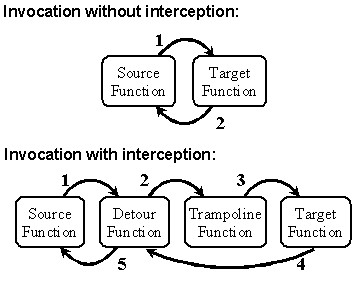
\includegraphics[scale=0.7]{sections/background/attacks/fig_detours.png}
	\caption{This figure shows the change in control flow of a detoured function \cite{detours}}
	\label{fig:detours}
\end{figure}


\paragraph{Buffer overflows}
Buffer overflows are among the most severe security problems of modern applications and are introduced by simple programming errors that weren't previously found in quality assurance steps. Even though they are hard to find, once used they allow the attacker to hopefully execute arbitrary code or in a less worse case just revealing too many information about the memory contents. One of the most severe examples of the past was the so called "Heathbleed bug" which affected millions of servers worldwide, as it was present in the much used OpenSSL library. Even though the attacker couldn't execute code directly, he was able to get sensitive information about the SSL certificates private key and thus break any security put in place by the SSL protocol.